\newpage
\section{3次元キャビティ流れ問題}
二層流解析を導入したプログラムに対して、二つの流体が同じパラメータの場合に単層の流れの結果と同じになることをキャビティ流れを解くことにより検証した。

\subsection{解析条件}
Figure \ref{fig:3d-cavity-mesh}に解析メッシュを示す。メッシュは四面体$1$次要素を使用した。解析領域の大きさは$[0, 1]\times[0,1]\times[0,1]$である。上面に速度のディリクレ境界条件として$u_{y}=1.0$を与えて、それ以外の面には滑りなし境界条件を与えている。
\begin{figure}[H]
	\centering
	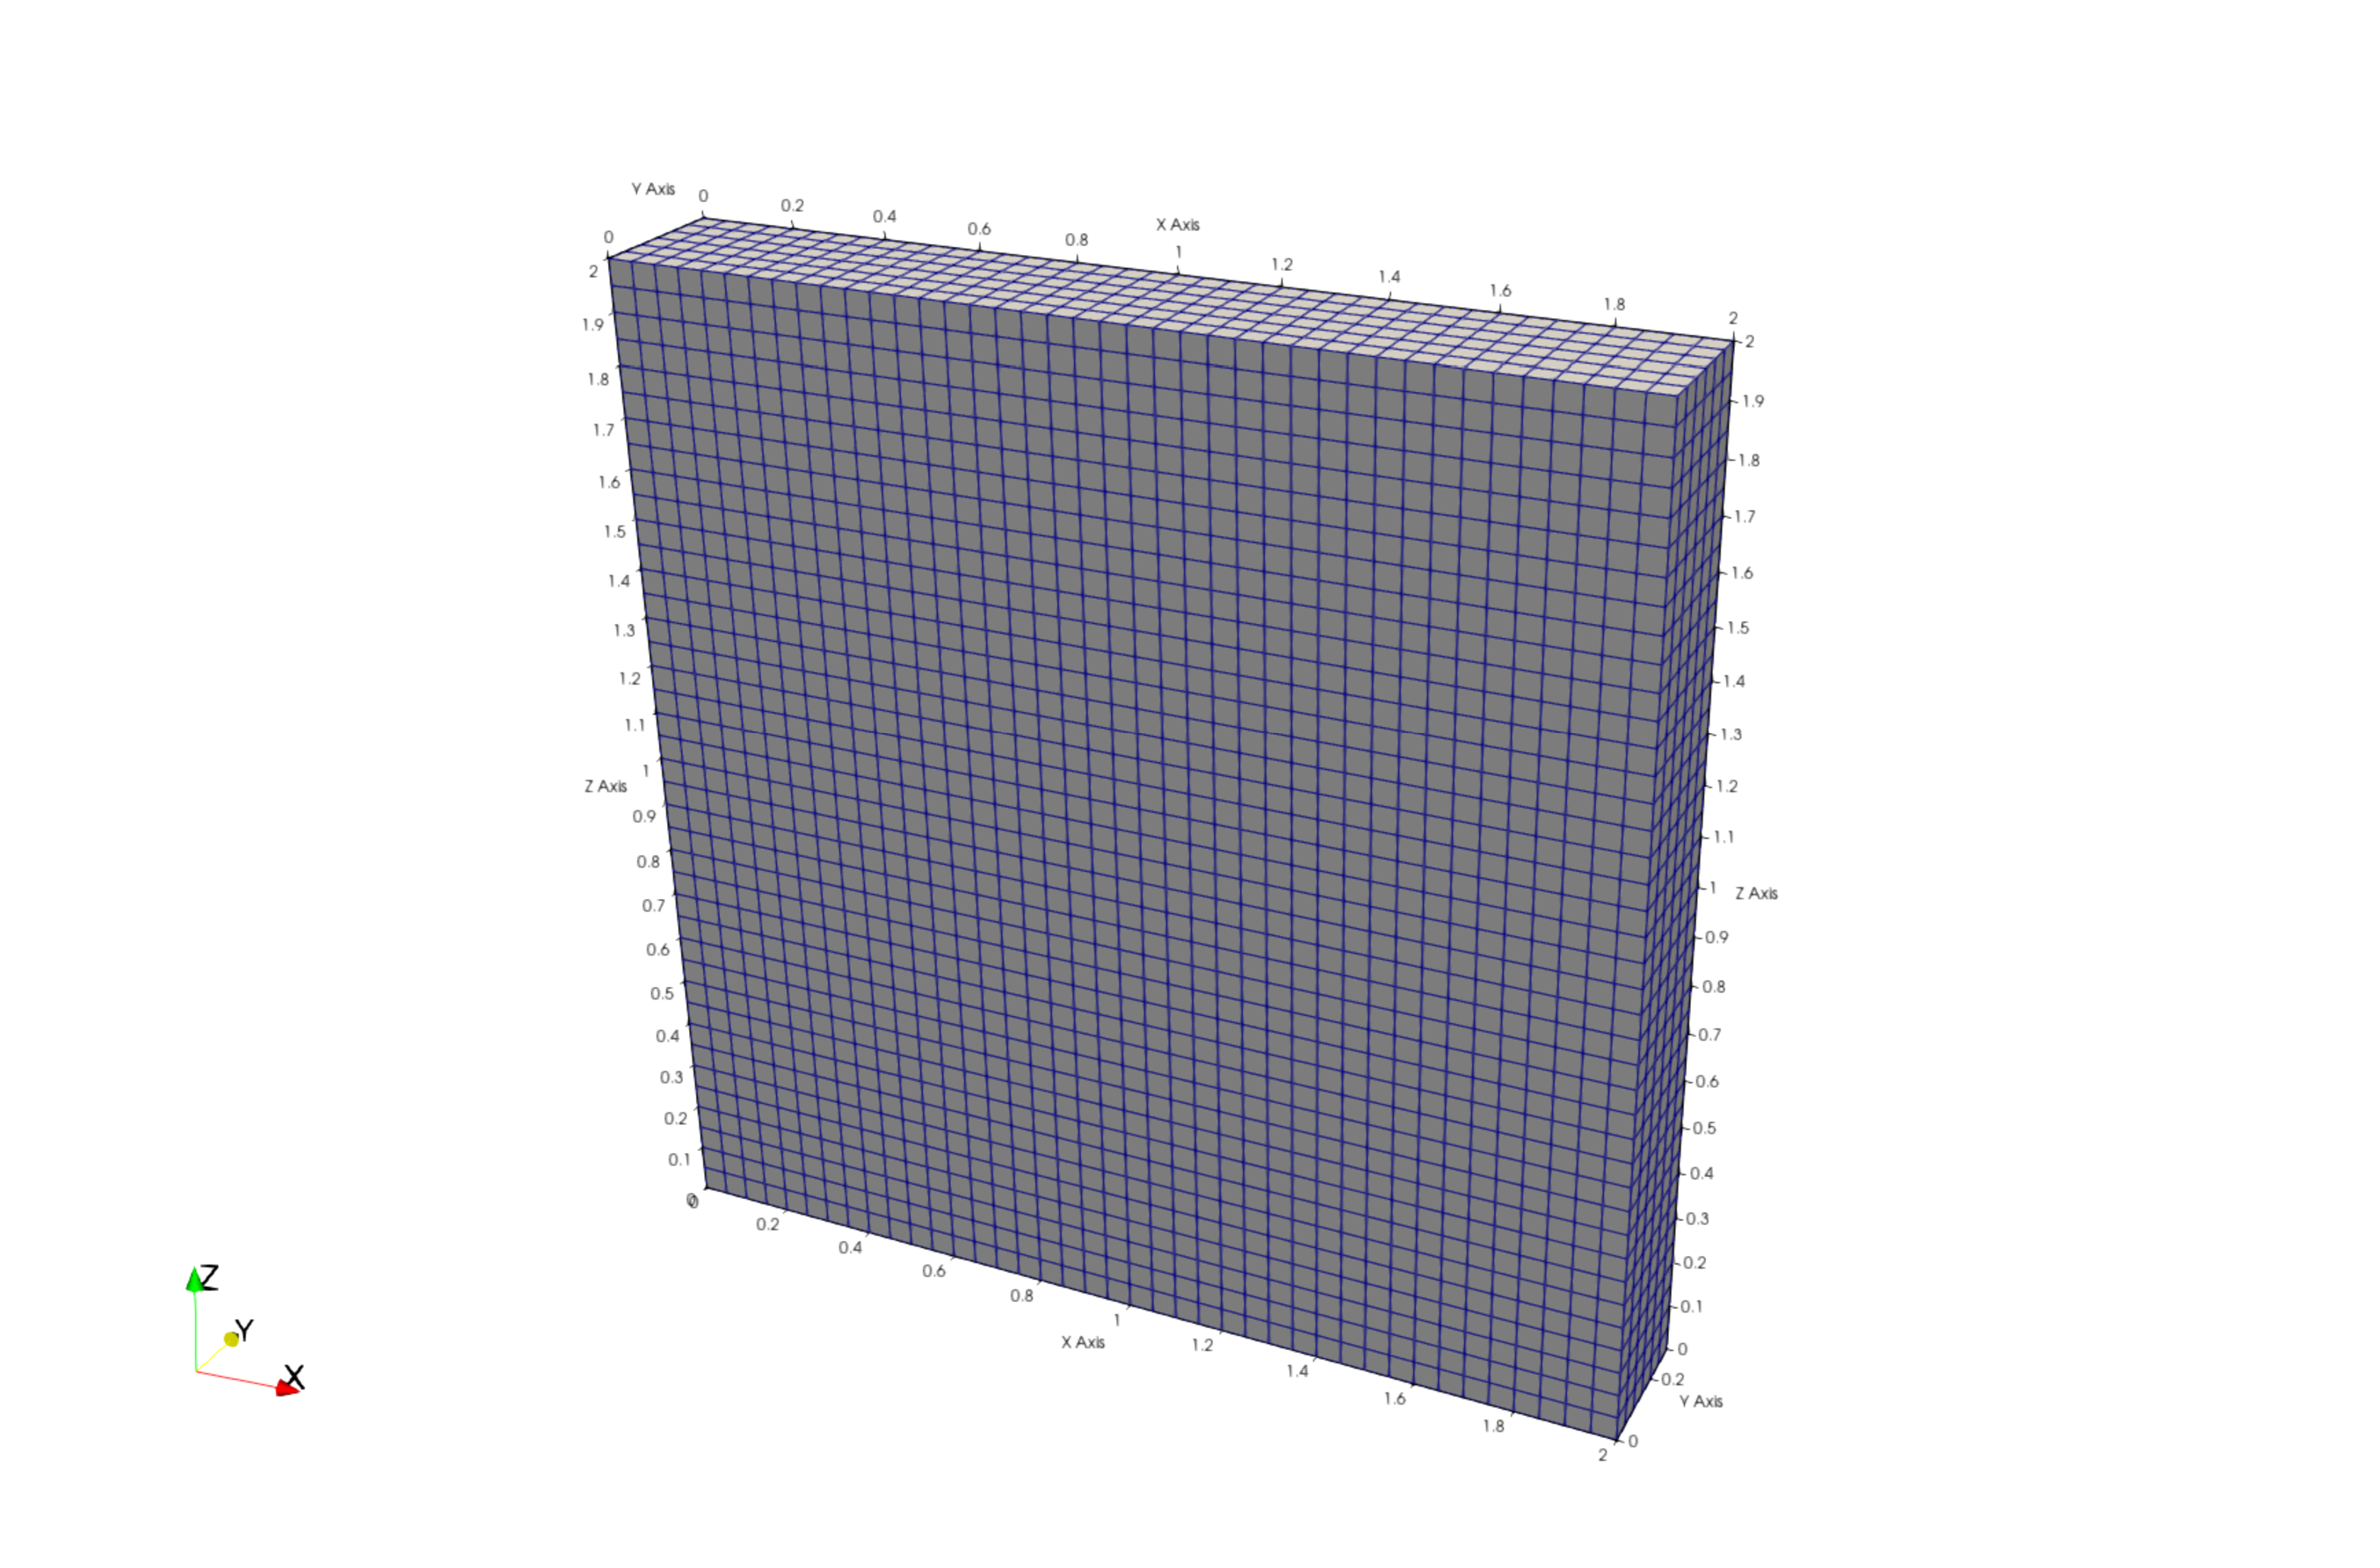
\includegraphics[width=10truecm]{pics/3d-cavity/mesh.pdf}
	\caption{解析領域のメッシュ}
	\label{fig:3d-cavity-mesh}
\end{figure}

Table \ref{table:fluid-ml-cavity-parameter}に解析パラメータを示す。
$z=0.5$の面を境界として$z<0.5$の領域を流体1、$z>0.5$の領域を流体2としている。
\renewcommand{\arraystretch}{1}
\begin{table}[H]
	\centering
	\caption{解析パラメータ}
	\begin{tabular}{cccccc}
		\hline
		Test case & $\rho_1$ & $\rho_2$ & $\mu_1$ & $\mu_2$ & $\mathrm{g}$\\
		\hline 
		Case$1$ & $1$ & $1$ & $0.01$ & $0.01$   & $0$ \\
		\hline         
	\end{tabular}
	\label{table:fluid-ml-cavity-parameter}
\end{table}
\renewcommand{\arraystretch}{1.0}

\subsection{解析結果}

Figure \ref{fig:3d-cavity-result-levelset}にレベルセット関数の時間変化を示す。
\begin{figure}[H]
	\centering
	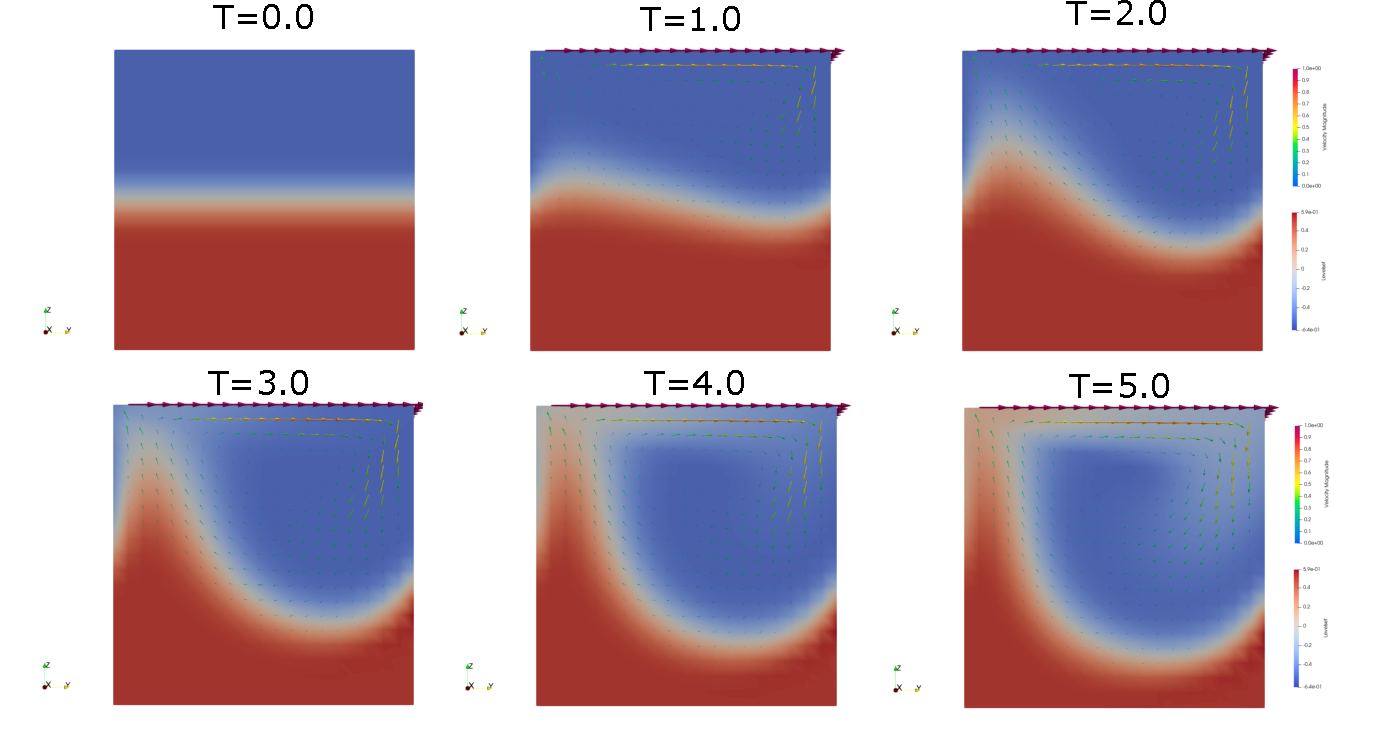
\includegraphics[width=18truecm]{pics/3d-cavity/levelset_velocity.pdf}
	\caption{二層キャビティ流れのレベルセット関数の時間変化($x=0.5$における断面)}
	\label{fig:3d-cavity-result-levelset}
\end{figure}

Figure \ref{fig:3d-cavity-result-velocity-pressure}に流速と圧力分布の結果を示す。
\begin{figure}[H]
	\centering
	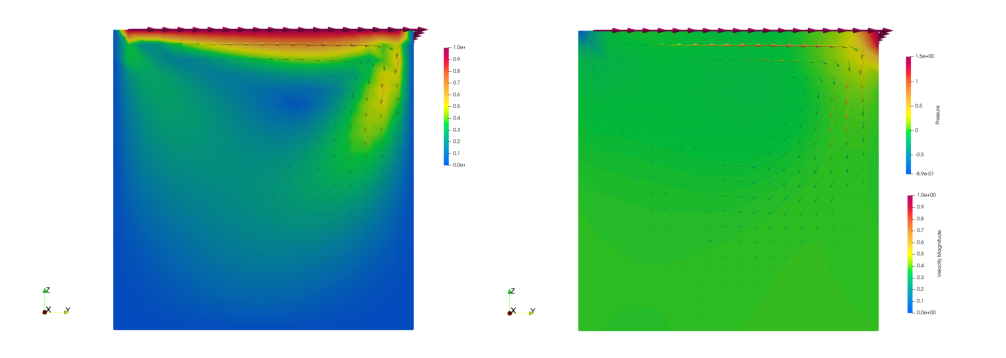
\includegraphics[width=18truecm]{pics/3d-cavity/velocity_pressure.pdf}
	\caption{二層キャビティ流れの速度と圧力分布($x=0.5$における断面)}
	\label{fig:3d-cavity-result-velocity-pressure}
\end{figure}

\begin{figure}[H]
	\centering
	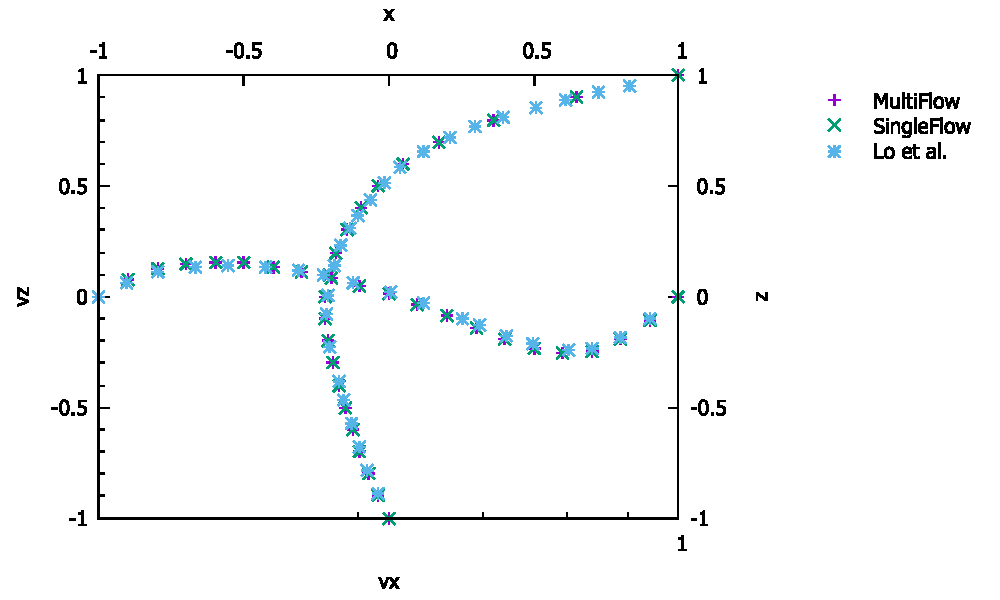
\includegraphics[width=18truecm]{pics/3d-cavity/velocity_graph.pdf}
	\caption{二層キャビティ流れと一層キャビティ流れの速度分布の比較によるプログラム検証$(T=30.0)$}
	\label{fig:3d-cavity_velocity_graph}
\end{figure}

Figure \ref{fig:3d-cavity_velocity_graph}より、単層流の場合と二層流の場合で速度分布が一致しており、また参考文献\cite{Lo2005}の結果ともよく一致しているため、プログラムの妥当性を検証できた。